\section{Approche}


Dans un premier temps, nous avions une petite liste de phrases (5 par langue) que nous avons observé pour faire ressortir une structure générale. Ce temps fut notre brainstorming, et nous a aussi servi à réfléchir au processus global. \\

Ensuite, nous avons choisi un code à utiliser pour les POS. \\

Puis seulement, nous avons commencé à programmer. L'automate fut rapide à mettre en place, de même que les différentes fonctions. \\

L'automate est de la forme :

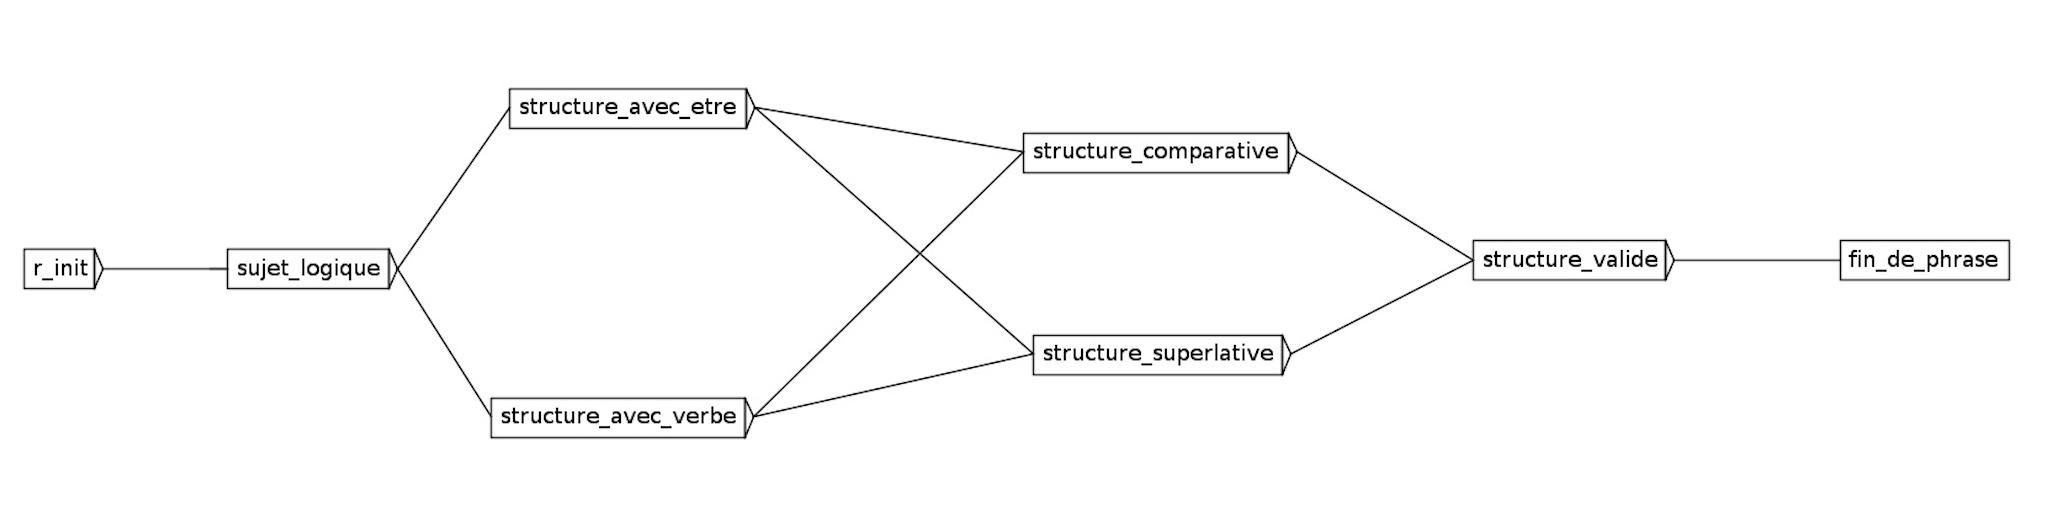
\includegraphics[width=1\linewidth]{./chap/img/dfa.png} \\

La plus grande partie du travail fut celle concernant les transitions. Elle a pris plus de 75\% du temps. \\

Puis ces derniers jours furent consacrés au nettoyage du code, et à l'écriture de ce rapport. \\

%-------------------------------------------------------------
\newpage
\section{Liste des problèmes}

Voici la liste des problèmes rencontrés. Ils sont présenter par ordre chronologique du plus ancien au plus récent. \\

{\small{
\begin{tabular}{|P{1cm}|m{7cm}|m{7cm}|}
\hline
\textbf{Num} & \textbf{Problème ou questionnement} & \textbf{Solution ou réponse} \\
\hline \hline
1 &  Sur quelle base doit-on fonder notre raisonnement ?
& Nous avons pensé que les \textbf{POS} étaient plus indiqués. Dans de rares cas, nous avons aussi utilisé le lemme. \\
\hline
2 & Comment formaliser une structure comparative ou superlative ?   
& Par l'\textbf{observation}, et en avançant pas à pas. \\
\hline
3 &  N'avons-nous pas besoin d'avoir des informations sur les mots et les phrases ?
& Si, nous nous sommes appuyé sur \textbf{treetagger}. \\
\hline
4 & Comme utiliser le même automate pour les deux langues ?
& Heureusement, le français et l'anglais ont des structures assez similaires, dans ce cas précis au moins. Il a seulement fallu prendre en compte le fait que le tagger analyse de manière plus fine en anglais. D'où l'utilité du fichier \textbf{l3\_pos.py}. \\
\hline
\end{tabular}
}}

